\documentclass[a6paper,hidelinks]{article}
\usepackage[margin=5mm]{geometry}
\usepackage{hyperref}
\usepackage{graphicx}
\graphicspath{ {./images/} }

% This defines a "namedlabel" command which allows you to reference
% named items in a description.
%
% Like this:
%
% Here's what an S thing is: \ref{itm:srt_S}
% \begin{description}
%	\item[\namedlabel{itm:srt_S}{S}] -
% \end{description}

\makeatletter
\def\namedlabel#1#2{\begingroup
    #2%
    \def\@currentlabel{#2}%
    \phantomsection\label{#1}\endgroup
}
\makeatother


\begin{document}

\tableofcontents

\section{Welcome to Pocket Dungeon!!!}
Pocket Dungeon is what I have come to call a ``stealth-game'' or ``ninja-game''. What that is, is a game that can be played out in the open without people knowing you are playing a game. Pocket Dungeon at its core is a Dungeon generator (the DunGen system) and slimmed down Dungeon crawler. The cool part about this, is this game also serves as a tutorial on how to stealth-game using items you will find (or would not look out of place) on your office or school desk. Pocket Dungeon is completely free to print and play, but if you enjoy the game and would like donation information, it can be found in the FAQ at the end.

The goal in Pocket Dungeon is very simple:  Enter a dungeon, kill lots of stuff, get phat lewt, bring death to the Boss and try to avoid Death's clammy grip. And don't get caught by your boss or coworkers while doing it!

\subsection{License, Authorship, and Contributors}

This was found here: \url{https://www.boardgamegeek.com/filepage/42518/pocket-dungeon} and was released under the creative commons license: \url{http://creativecommons.org/licenses/by-nc-sa/3.0/}.  It was posted in 2009.

Designer: Jonathan Gilmour

Typeset in \LaTeX\ by Martin VanWinkle.

\section{Setup and the Road Less Traveled}
Now my friend let me show you the way of lost productivity. It’s time to make our stealth gaming supplies. You may skip this section if you plan on using dice  along with the Deluxe version. If you go that route, every time you see {\em flip} in the manual, pretend it says {\em roll}.

Here is what you will need:

\begin{itemize}
  \item 1 copy of Pocket Dungeon printed off, and folded using the folding guide on \url{http://www.pocketmod.com/howto/}
  \item 1 small stack of post-it style notes. The really little ones if you can find them for added stealth\ldots Big ones should work too though.
  \item 1 Pencil. I like mechanical you can use old fashion, let your conscience be your guide on this one.
  \item 1 Slacker attitude and a real commitment to avoiding work.

\end{itemize}

Now, do the following steps in order:
\begin{enumerate}
\item Print off the Pocket Dungeon sheet, and fold it up really nice. Spend a few minutes on this. You really didn't need to get that report done any time soon, did you? Folded up proper? It should look like a ToDo list on the front, followed by the (patent-pending) DunGen page, and then a page of graph paper, and then another DunGen chart and associated graph. The two pages before the last are extra charts and character generation information. Each Pocket Dungeon sheet will contain enough space for two Dungeons.
\item Take your stack of post-it style notes. Flip to the very last one. Write 1 in the bottom right hand corner. Flip to the next sheet. Write a 2. Repeat this process until you reach six. Are you there yet? good. Now flip to the next sheet, and start over at 1. Repeat 1-6 until you are about 3/4ths of the way through the stack.
\item Now go back to the bottom note and on the bottom left start at 1 and then progress to 8. All the way up the stack. Take your time. This will become your
stealth dice. If you are REALLY avoiding work, you can also throw a 1-20 in the middle and play some DnD at your desk.
\item Take the stack of post-it style notes. Press them firmly against the desk. Put your thumb on the bottom right hand corner. Now riffle through the sheets and stop somewhere. See what we just did? All the random joy of a d6 with none of the clanky clank. The other corner is a d8. These are the only two dice you will need for Pocket Dungeon. If you ever need a d4, just use 1-4 on the d8 side, and then again 5-8. Sneaky eh?

\end{enumerate}

\section{The Game as She is Played}

Now it is time for me to introduce you to the patent pending DunGen system.

\subsection{The DunGen System}

\begin{figure}[!]
\caption{The DunGen System}
\label{fig:the_dungen_system}
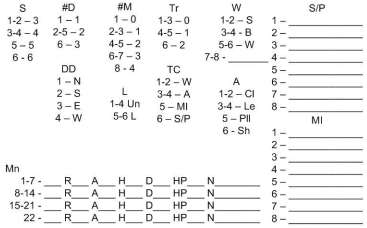
\includegraphics[width=0.8\linewidth]{dungen_system_snip.png}
%\tiny{
%\begin{tabular}{c c c c c c}

% S Table
\begin{tabular}{| r | l |}
\hline
\multicolumn{2}{|c|}{\ref{itm:srt_S}} \\
\hline
1-2 & 3 \\
3-4 & 4 \\
5 & 5 \\
6 & 6 \\
\hline
\end{tabular}

&

% #D Table
\begin{tabular}{| r | l |}
\hline
\multicolumn{2}{|c|}{\ref{itm:srt_nD}} \\
\hline
1 & 1 \\
2-5 & 2 \\
6 & 3 \\
\hline
\end{tabular}


&

% #M Table
\begin{tabular}{| r | l |}
\hline
\multicolumn{2}{|c|}{\ref{itm:srt_nM}} \\
\hline
1 & 0 \\
2-3 & 1 \\
4-5 & 2 \\
6-7 & 3 \\
8 & 4 \\
\hline
\end{tabular}

&

% Tr Table
\begin{tabular}{| r | l |}
\hline
\multicolumn{2}{|c|}{\ref{itm:srt_Tr}} \\
\hline
1-3 & 0 \\
4-5 & 1 \\
6 & 2 \\
\hline
\end{tabular}

&

% W Table
\begin{tabular}{| r | l |}
\hline
\multicolumn{2}{|c|}{\ref{itm:srt_W}} \\
\hline
1-2 & S \\
3-4 & B \\
5-6 & W \\
\hline
7-8 & \\
\hline
\end{tabular}

&

% S/P Table
\begin{tabular}{| r | l |}
\hline
\multicolumn{2}{|c|}{\ref{itm:srt_SP}} \\
\hline
1 &  \\
2 & \\
3 & \\
4 & \\
5 & \\
6 & \\
7 & \\
8 & \\
\hline
\end{tabular}

\\

&


% #DD Table
\begin{tabular}{| r | l |}
\hline
\multicolumn{2}{|c|}{\ref{itm:srt_DD}} \\
\hline
1 & N \\
2 & S \\
3 & E \\
4 & W \\
\hline
\end{tabular}

\end{tabular}

%}
\end{figure}

Take a look at figure \ref{fig:the_dungen_system}.
Looks like a just a random bunch of letters and numbers huh? I like to call this game camouflage. But you are a smart gamer; you should be able to make sense out of this after I detail how to use it. Mastering this system
should give you a sense of accomplishment, hopefully more so then the work you are avoiding doing by playing games. First, before I get into what the letters mean, let's look at how to read the numbers, shall we?
When you see something like figure \ref{fig:shortened_roll_table}:

\begin{figure}[h]
\caption{Shortened Roll Table}
\label{fig:shortened_roll_table}
\centering
\begin{tabular}{| r | l |}
\hline
1-3 & X \\
4-5 & Y \\
  6 & Z \\
\hline
\end{tabular}
\end{figure}

Read it like this: On a roll of 1 to 3, do X. On a 4 or 5, do Y. And If I roll a 6,
then I will do Z.

Simple enough.

% Here's what an S thing is: \ref{itm:srt_S}

\subsubsection{These Letters, They Must Mean Something!}

\begin{description}
\item[\namedlabel{itm:srt_S}{S}] - Size of the room that you are entering. This is how many squares it should take up. But what shape you ask? I don't care. This is part of the fun of Pocket Dungeon, using the random rolls to make your dungeon. Roll a 3, make a room that’s 4 squares. It can be a hallway, a square room, or some other crazy shape. The only rule while drawing rooms, is that it cannot result in there being squares without rooms trapped somewhere on the map.

\item[\namedlabel{itm:srt_nD}{\#D}] - Number of added doors. Obviously the room already has one door, you walked through it, right? Since you are entering a room for the first time, this is how many other exits you see. Where do you put them? Don't put it right next to the one you came in from, unless it would lead to a different room then the one you just came out of. Still can't figure it out, then use the handy Dd chart.

\item[\namedlabel{itm:srt_L}{L}] - Door/Treasure lockedness (yeah, I know it’s not a real word). Is the door, locked, unlocked, or some other mystical quantum state? Only this chart can tell. This is to be used both when putting down doors (ONLY for rooms with more than 1 door being added), and chests. There are several different ways to open a locked item: Warriors can Bash, Thieves can Pick Lock, Wizards or Rangers can use the spell Knock or you can use then discard a Key if you have one.

\item[\namedlabel{itm:srt_DD}{DD}] - Door direction. This is for the times when you can't decide which side of the room to stick a door on. You can also use this table for other things, like deciding where to put a treasure, or which way to go young man.

\item[\namedlabel{itm:srt_nM}{\#M}] - How many monsters are in the room? This tells you! Roll it up, slap them down. I use X's, you can draw whatever you want. Where do you put them in the room? I don't care! You choose!

\item[\namedlabel{itm:srt_Mn}{Mn}] - What kind of monsters are they? This chart has some differences. It has a few \underline{\hspace*{1cm}}'s. You will need to fill this out before you start the dungeon. If you are currently playing, and referring back to this because you don't know what the \underline{\hspace*{1cm}} is for, then you failed to read the instructions BEFORE you started playing.

Want to fight Goblins, Orcs, and Trolls?  Then put a G on the first line, O on the second, and T on the third. Want to fight the undead? How about S, Z, G for Skeletons, Zombies, Ghouls? The only rule is they should go from easiest to toughest, as the rolls should favor more of the easier ones.

There is a string of information after the monster type. We will get into that later.

\item[\namedlabel{itm:srt_Tr}{Tr}] - It's not a dungeon crawl without treasure! This is how many chests are in the room. Each chest has one item in it. What kind of item? Roll it out on the next chart when you open it! Make sure you checked the chest for lockedness before trying to open it.

\item[\namedlabel{itm:srt_TC}{TC}] - Treasure Contents. This is the goodies in the chest. W(eapon), A(rmor), M(agic)I(tem), S(croll)/P(otion). Roll to see what you get on the appropriate table.

Note that S/P has several blank spots that you can choose items from the list at the end of the instructions and fill in. Once you roll the Treasure Contents, Roll again on the equipment list for the appropriate type.

\item[\namedlabel{itm:srt_W}{W}] - Weapon

\item[\namedlabel{itm:srt_A}{A}] - Armor 

\item[\namedlabel{itm:srt_SP}{S/P}] - Scroll/Potion

\item[\namedlabel{itm:srt_MI}{MI}] - Magical Item

\end{description}

There is also a little empty area on the right side, feel free to make your own charts to cover any special circumstances or charts you may want to add in.

\subsection{So I'm in this dungeon, going around killing all these goblins, and I’m like Whaaats the deal?}
Now that you are ready to start generating your dungeon, it is time to decide what the goal of it will be. As with most of the rest of the game, I will provide you with some examples, and framework, but the decision remains yours to make.

The default goal is to find the exit and leave the dungeon. Here’s the rub. The exit is locked, and it’s not pick-able or bash-able. Who has the key?

\subsubsection{The Boss!}

 Where is the boss? Waiting for you in his lair. Who’s the boss? Hopefully not Tony Danza! So when you start creating your dungeon, put the exit on the side opposite of your entrance. When you finally place the boss in his lair, he obeys a couple different rules. He will not leave the room he is spawned in, and you cannot attack through the door of his lair. Boss monsters do not need to be fought immediately, as you may need to get some better equipment before you can kill him.

\subsection{Quests}
There will be pre-made scenarios that you can download that have more complex goals. They will feature specific instructions and rules. Be sure to read through them before beginning your adventure.

So that wraps the basics up. Pretty complicated huh? So let’s try one out together (see the next section),
and then I will tell you how to kill stuff via the super simple combat system (also patent pending).

\subsection{Putting it all Together}

\begin{quote}
My hero enters the dungeon of despair! I draw a flat line across one square on the bottom of the graph and put a
door on it. This is the entry way to the dungeon. I also draw the exit on the opposite side of the dungeon. *flip* 4. I look it up on the S chart, and 4 is room covering 5 squares.

I draw a reverse L shaped room, two across against the bottom of the graph. and then up three on the right side. 5 Squares in all. I place my starting door on the entryway I picked earlier. I draw my doors like $| |$ through a wall. Locked doors are $|\backslash|$.
*flip* 5. So, 2 more doors. I add one on the north east side and one on the north west side. *flip* 3. The second one is unlocked. Awesome!

Any bad guys? *flip* 2.  So there is just 1 baddie here. What is he? Lets looks at the DunGen, it says Kobolds in rooms 1-9, so it’s a kobold (there is a note for him, we will get to that in a bit) wheee!  Is he guarding anything? *flip* 5.  One treasure, tucked against the far north wall of the corridor.

\end{quote}


Now it's time to do the dance, so on to Character creation, and combat. We'll come back to Mr. Kobold McKoboldski (That is his name, scouts honor, I rolled it on one of my custom tables) in a bit.

See the end of the manual for example monsters to populate your dungeons with.

\section{So You Want to be an Adventurer?}

\subsection{Character Generation}
Character generation in this game is as simple as everything else. Assign some points to your stats, pick some starting equipment and start crawling those dungeons.

The character stats are as follows:
\begin{description}

\item[S(trength)] - Determines your hero's Physical fortitude, along with his prowess with weapons. S(trength) is the determining factor in most melee combat.
  \begin{description}
  \item[1-2] - May use Cloth armor, Daggers (including pair of daggers), iron knuckles, wands, and bows
  \item[3-4] - May use Leather armor, all other 1 handed weapons, and shields
  \item[5-6] - May use Plate armor and 2 handed weapons.
\end{description}

\item[D(exterity)] - How agile and quick your hero is. Dexterity is also used for combat with ranged weapons.
M(ovement) is half your D(exterity) rounded up. This is how many squares you can move in one round of combat. The lowest being 1 (the same speed as most monsters, uh oh!).

\item[W(isdom)] - The mental aptitude of your hero.

\item[A(ction)P(oints)] - Your hero gets 2AP for every point in wisdom. Your AP restores to half your max when you are out of combat. (No enemies in the current and adjacent revealed rooms).

\end{description}

S,D,W are determined by distributing 9 points (with no more than 5 points in a single stat) among the 3 attributes. Stats may be raised later by expending  Fudge Points, or temporarily through the use of potions and scrolls.

HP varies for each class; see the next section for details.

Finally, choose your profession. Will you be a mighty W(arrior), or a shifty T(hief), a foresty R(anger) or a powerful (Wi)zard? Here are the benefits of each class.

\subsection{Warrior}

(HP is 10 + d8) May not use spells or scrolls.

\begin{description}

\item[Bash - 1AP] - bash a locked door or chest. Succeeds on 5-6. +1 to the roll for every 3 points of Strength
\item[Jump - 1AP] - May jump over an enemy into an empty space. Succeeds on 5-6
\item[Precision Strike - 1AP] - Your attack this round gets +2H but -1D
\item[Knockdown - 2AP] - You knock your opponent down immobilizing them for 2 turns.
\item[Whirlwind - 2AP] - Attack all enemies adjacent to your hero. Must make a successful attack roll on the enemy with the highest Armor.
\item[Battle cry - 3AP] - You let out a piercing scream, all monsters attacking you get -1 to their rolls to hit you for the next two rounds of combat.
\item[Flurry of Blows - 4AP] - You rain blows down on your opponent, you may make twice your normal amount of attacks this turn.


\end{description}

\subsection{Thief}

(HP is 8 +d8) May not use spells, but they can use scrolls. Thieves may only use Cloth and Leather Armor. They may also only use 1Hnd weapons and Bows.

\begin{description}

\item[Pick Lock - 1AP] - May attempt to pick a treasure chest or door lock. Succeeds on 5-6. +1 to the roll for every 3 points of Dexterity.

\item[Sneak - 1AP] - May attempt to pass through a room unnoticed. Must roll 3-6 to succeed. Check for every monster whose LOS you pass. Once you fail a sneak check, you may not sneak again in the current room.

\item[Blinding dust - 1AP] - You throw a handful of dust in target enemies eyes. They receive -1 to their combat roll this turn.

\item[Critical Strike - 2AP] - Deal Double damage to a monster. Must make a successful attack roll.

\item[Vengeful Strike - 2AP] - You may only use this attack against an enemy that has just dealt damage to you. Your next normal attack cannot miss.

\item[Blade flood - 3AP] - You may make your normal amount of attacks on each adjacent enemy. Each attack must be rolled separately.

\item[Backstab - 4AP] - You must make a successful attack while sneaking to use this ability. Kill target adjacent non-boss enemy. If your attack fails, you lose your next 2 rounds of combat.

\end{description}

\subsection{Ranger}

(HP is 8 +d6) May use spells (May only have one equipped at a time) and scrolls. Rangers may only use Cloth and Leather Armor. They may also only
use 1 handed weapons and bows.

\begin{description}

\item[Quick Strike - 1AP] - You may both make an attack and move this round of combat.

\item[Aimed Shot - 1AP] - Requires bow equipped. Instead of attacking this turn, you may focus your energy on piercing an enemies defenses. For each round spent in this manner, you gain 2H on your next attack. For every round past the first, you also gain +1 damage.

For example if you spend 3 rounds, and 1AP per round, on your fourth round you make an attack with a +6 bonus to Hit, and +2 bonus to Damage).

\item[Striders Legs - 1AP] - You call upon your years of navigating treacherous terrain, add 2 to your movement rate for 3 turns.

\item[Cripple - 2AP] - Targets movement is reduced by half. If the targets movement is already 1, it may only move every other turn.

\item[Bear Trap - 2AP] - Makes a square of the dungeon impassable for 2 turns.

\item[Triple shot - 3AP] - Requires bow equipped. You fire off three shots in rapid succession. Each shot beyond the first gets -1 to your hit roll.

\item[Focused Speed - 4AP] - Double your Dexterity for 2 turns.

\end{description}

\subsection{Wizard}

(HP is 6 +d6) May have two spells at a time memorized. This is because of their huge amounts of Wisdom, or the notepad they carry around with them. May use spells and scrolls. Wizards may only use Cloth armor and may not use shields (Gotta keep those hands free for spell casting).

\begin{description}

\item[Dark Rituals - 0AP] - You may take 4 damage to recover 4AP.
\item[Spell Recall - 1AP] - You may swap out one memorized spell with one in your spell book during combat.
\item[Empower Spell - 2AP] - May double one aspect of your next spell. May choose Range, Damage, or Hit Bonus
\item[Overload - X AP] - For each AP spent, each turn you regenerate X AP per X turns (i.e.: 1AP - each turn you regenerate 1 AP for 1 turn; 2AP - each turn you regenerate 2AP for 2 turns; and so on ..), when Overload wears off, take 1 damage for each AP you still have.
\item[Etherlink - 4AP] - Regenerate 2AP per turn. Ends, if you perform any other action besides casting spells.

\end{description}

\subsection{Sample Character Generation and Battle}

I’ll be calling my hero Meathead the Squishy.
So first I assign my stats, he is S1 D3 W5. I wonder what class I
should choose. How about (W)izard? Let’s hope he doesn’t
ever need to run away or come face to face with anything too
nasty. A quick *flip* and I can write down his health as 8, and I
put his movement down as 2. I also put down that he has
10AP.
I'm going to choose MM as his spell and 2 P(otions) 1 Health
Potion, and 1 AP potion.
So now I have my adventurer.
Here is a picture of the our first room:

\begin{figure}[h]
\caption{Meathead the Squishy's First Battle}
\label{fig:meatheads_first_battle}
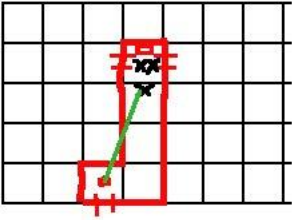
\includegraphics[width=0.8\linewidth]{meatheads_first_battle_vs_kobolds.png}
\end{figure}

The green line is Line of Sight, which obviously fails. Everyone
knows you can’t cast magic missiles around corners, that
would just be silly.
So combat goes like this
Round 1 – I move one square right, the Kobold moves one
square down towards me.
Round 2 – I unleash my two MMs *flip*5 + 5 +1 (flip, plus my
W(isdom), plus MMs H(it bonus) *flip*1 +5 + 1. The first one
hits! (The Kobold has A8, so I have to beat that) and do the D1
listed at the end of the instructions (I also wrote that info
down with my character stats). The Kobold, and his friends
moves down again closing the gap between us.
Round 3 – Pew Pew! *flip*3 +5 +1 *flip*2+5 +1 One hit, one
miss. He is mad! *flip*4 for his attack. I take 2 damage.
And it goes on like this. In the end, Meathead is triumphant
and gets to open the chest. *flip*2, unlocked! From here all I
need to do is find out what kind of treasures await me in the
chest, and decide which door to go through.

\subsection{Starting Eqipment}
Now, pick your starting equipment. You get {\em one} W(eapon) or S(pell), and {\em either} 2 P(otions) or 1 Cl(oth armor).

The weapon and spell stats are simple. R(ange) D(amage) H(it bonus) and Hnd(handedness). Only Wizards and Rangers can have spells. Each weapon will detail in the equipment list what skill it uses for its attack roll, along with any special effects it has. See the last page for a list of equipment.

\subsection{In the eternal words of Leroy Jenkins, ``Let's do this thing!!!''}

Now its time to kill Kobold McKoboldski.

First, let’s look at his stats on our sheet I would have written down before hand:
\begin{itemize}
\item 1-9 Kobolds - M1 R1 A8 H1-2 D2 HP3 Note:+2 Per Room (after you roll to spawn, add two.)
\end{itemize}

Let's take a second to break down all the information crammed in there.

\begin{description}

\item[1-9 Kobolds] - That’s what got us our guy in the first place. Every single room between 1 and 9 will contain kobolds.

\item[M(ovement)1] - Kobolds move one square each turn of combat.

\item[R(ange)1] - The monster's range. This guy can only hit stuff in the square next to him.

\item[A(rmor)8] - This is the number I am going to have to beat for my attack to land. I'll flip a d6, add my appropriate skill and any bonuses my spells or weapons give me. If it is higher than their A I hit, lower or equal misses.

\item[H(its)1-2] - This guy is a brawler. On a d6 flip of 1-2 he hits you and does his damage.

\item[D(amage)2] - He will poke you with his sword for 2HP. You armor ``soaks'' up its AC in damage once per round, so use it wisely.

\item[HP3]  Same as you, he only has a certain amount of life force. Spill it on the ground to defeat him! I use hash marks next to them on the map to track this. Feel free to use your desk calendar, your top post-it style note, or write on your hand.

\item[N(otes)] - Kobolds like go gang up, So after I roll for the number in the room, I add 2 to it. So I will actually be fighting three of the little buggers, instead of the one I expected.

\end{description}

\section{Notes and Details}

By now you should have a good enough idea how to play. Here are a few other little notes and details.

\subsection{Combat}

\begin{itemize}

\item You may NOT attack through doors.

\item You can only have one monster in each square around you at a time. In squares farther away, you can clump then together, but you can’t have more
than 4 monsters attacking you at once. Any additional monsters will line up behind them like in old Kung fu movies.

\item For every 5 enemies you kill, mark down a ``fudge'' point. You can use these fudge points to fudge a roll by plus or minus one. Once a point is used, it is gone forever. You can also save your fudge points and trade in 3 of them for a permanent +1 to any stat, or +3HP.

\item Each turn of combat you have three choices. Move, Fight, or Use a scroll. You can use a potion AND do any of those things as well. Enemies behave with a very predictable pattern. If they are far away and have no range attack, they move closer. If they are close enough to attack, then they do it. Spells, skills, and other effects can override this.

\item Out of Combat is defined as: No monsters are present in the current room, or any adjacent revealed rooms.

\item Armor “soaks” its Armor value in damage each round of combat. So if you get hit by 2 Kobolds in a round of combat, and you have cloth armor, then it
would absorb 1 of the 4 HP of damage you would need to take.

\item Shields can only be used if you have a 1 Handed weapon equipped. They cannot be used with two handed weapons.

\end{itemize}

\subsection{Equipment}

\begin{itemize}
\item For every 5 rooms you have explored, you may add one point onto a new item when you find it. For example: If I open a chest in room 11 and it has a
sword, I have two “bonus” points I can add to the weapon I find. So a base S(word) is R1 D2 H0. I can distribute the points any way I want, so I decide
that this sword is going to be R1 D3 H1. This is to represent the better items deeper into the dungeon. The cost is the same (2 bonus points). Exceptions
to this rule are:

\begin{description}
\item[Armor] - You may only increase armor 1 point for every 15 rooms, but you may spend unspent bonus points on aspects, these are magical things about a piece of armor, you may only have one of each aspect assigned to any piece of armor. You may also use the aspects from the armor table below on weapons. They cost 2 bonus points each, and are follows:
\begin{description}
\item[Bears Strength] - +1 to Str while this armor is equipped.
\item[Weasels Quickness] - +1 to Dex while this armor is equipped.
\item[Mountains Knowledge] - +1 to Wisdom while this armor is equipped.
\item[True Striking] - +1 To Hit while this armor is equipped.
\item[Hardiness] - +3 to HP while this armor is equipped.
\item[Youths Vigor] - +4 to your max AP while this armor is equipped.
\end{description}

\item[Spells] - Bonus points can only be spent on Combat spells. You may also increase spells range with bonus points, along with the standard D and H.

\end{description}

\item You may swap spells from your spell book, to your equipped spell slots as long as you are out of combat. To learn new spells, you will need to find spell books in treasure chests. See the description of Spellbook in the Magic Items section at the end of this manual.

\end{itemize}

\subsection{Monsters}

\begin{itemize}

\item Each room is considered a monster’s area. A monster will not leave his area unless there is a chance they will be able to catch you. So if your speed is greater than theirs, the monsters will not follow you outside of their area. If your speed is equal to or less than theirs, they will follow you until one of you are dead. If you run away from a monster (leave it behind in its room), when you return they will be fully healed.

\item The boss Monster is placed in the room number indicated on the DunGen chart. He does not need to be immediately fought, as you may need to explore a few more rooms until you can find equipment that is leveled enough to allow you to hit him. The boss monster will never leave his lair, and fully heals as soon as you leave.

\item When a room is completely cleared of monsters, you may roll to determine if the monsters have any loot on them. On 5-6 on a d6 you find one piece of salvageable equipment. Roll on the Treasure Type chart to determine what you find.

\item The DunGen system uses a scalar system for monster placement. Feel free to adjust this number to accommodate different crawl lengths. If you want a
longer dungeon crawl, then change it to 1-15. 16-31, 32-47, 50. Or even longer if you feel. You will notice the system varies between the PocketMod
version, and the Deluxe version, this is because the PocketMod version is intended for quicker play, so it has a slightly quicker set.

\end{itemize}

\subsection{Different Versions}

\begin{itemize}

\item The PocketMod version of the game features a lighter version of the DunGen system. The monsters do not have a Movement stat (they all move 1), and
there are blank lines to write in the Scrolls/Potions, and Magical Items you want. This is mostly because the deluxe version depends on an entire page of equipment for the treasure rolls.

\item The Deluxe version does not have any DunGen charts for Weapon, armor, Scrolls/Potions, or Magic Items. That’s because it’s on page two and should be printed on the back. The numbers are beside each item for your rolls. Convenient huh?

\end{itemize}

\section{M.U.F.A.Q. (Made Up Frequently Asked Questions)}

\begin{description}
\item[Q:]  The system for flipping the rolls seems pretty flaky. Can't I cheat by trying to hit the same spot in the note stack every time?
\item[A:]  srlsy? You want to cheat in a solo game. Sorry, you lose at life buddy. If you are not stealth gaming, feel free to use dice as well.
\end{description}

\begin{description}
\item[Q:]  This game is tooooo hard. I keep dying.
\item[A:]  That is very likely. A couple common causes:
\begin{itemize}

\item Are you using your Bonus Points to improve equipment when you find it? Remember, 1 BP for every 5 rooms.

\item Don't forget your Fudge Points. They can either be used to save you from a bad roll, or saved up and spent on character improvements.

\item Still dying? Try messing around ``under the hood''  of the game. Feel free to Distribute 10 points at character creation, or lower some of the
enemy stats in the DunGen (Likely candidates would be Armor and Damage, maybe HP). Feel free to experiment with the game and find out what works best for you. I personally love a good
\end{itemize}

\end{description}

\begin{description}
\item[Q:]  What?! Why are there so few weapons and cool stuff? I want to shop and do more stuff!! Where is my crafting and trade skills!?!?!??!? *head asplode*
\item[A:] Go play DnD.
\end{description}

\begin{description}

\item[Q:]  I just got fired for doing this at work.
\item[A:]   You used dice didn't you? And minis too huh? You wore your nerd-cloak. AND you made the guy in the next cubicle DM? Yeah.. Not really sure why you got fired, sounds normal to me.
\end{description}

\begin{description}
\item[Q:]  Fantasy games suck! Can I make it a Sci-fi Western Steampunk game?
\item[A:]  Sure! Substitute the weapons for other things like L for Lasersword and R for raygun. The monsters can be H(eadcrab), A(lien), R(obot-Steam driven) and the B can be a Giant mechanical spidery thing driven by cowboy space hobbits for all I care. The rooms are still rooms, just way more scifi and steampunky.
\end{description}

\begin{description}
\item[Q:]  What about character progression? Levels? anything like that?
\item[A:]  For every 15 monsters killed, you can raise a skill point or you HP, and if you carry your character between adventures, then that’s kind of like progress, right?
\end{description}

\begin{description}
\item[Q:]  I can't play a game without a REAL goal. All I'm supposed to do is kill stuff and loot?
\item[A:]  Well, I guess you could say the REAL goal was avoiding work.
\end{description}

\begin{description}
\item[Q:]  Is this it? What do you have planned down the road?
\item[A:]  Its still pretty early in development. I would eventually like to add some stuff that uses S(trength) and D(exterity) like traps or something, and some more weapons and possibly a weapon modifier system. And more spells. Everyone loves more spells, right? And probably some of the stuff from the next question too.
\end{description}

\begin{description}
\item[Q:]  I'm not creative at all. Can I have a list of Monsters and stats? How about spells I can switch out? Bigger lewt tables?
\item[A:]   Yes. Check the end of this manual, or print out the Deluxe version, which includes more equipment and more Monsters.
\end{description}

\begin{description}
\item[Q:]  What can and can’t I do with your game?
\item[A:]  Please don't resell this game as your own work, or alter it without attributing me (Jonathan Gilmour). Please DO feel free to upload additional content (premade quests and dungeons, etc) to board game geek for the community to enjoy.
\end{description}

\begin{description}
\item[Q:]  Sir you have pleased the pants right off of me with this fun and awesome game. I would like to return the favor. Is there anything I can do for you?
\item[A:]  Just the fact that people are enjoying my game is an awful big reward, but I know the feeling. You may send a donation to me via PayPal via my email address: jgilmour@gmail.com

If you rather send me a game or a package or just want to ask me a question or make a suggestion, then feel free to email me, or you can reach me on BGG at
\url{http://www.boardgamegeek.com/user/jgilmour} . I will be donating a portion of any proceeds to a local charity.
\end{description}

\begin{description}
\item[Q:]  I just bought this game from a website.
\item[A:]  This game is only distributed for FREE via www.boardgamegeeks.com. The webpage for the game is \url{http://www.boardgamegeek.com/boardgame/42361}.   If you found the game somewhere else, please contact me.  (Note; it was released under the creative commons license:
\begin{quote}
Pocket Dungeon is released under a Creative Commons Attribution-NonCommercial-ShareAlike 3.0 Unported License. So feel free to remix and share away! Find out more here: \url{http://creativecommons.org/licenses/by-nc-sa/3.0/}
\end{quote}

\end{description}

\section{Items}

\subsection{W(eapons)}

\subsubsection{Hand Axe}
R1 D2 H0 1Hnd (Attack Skill is Strength)

\subsubsection{Sword}
R1 D2 H0 1Hnd (Attack Skill is Strength)

\subsubsection{Dagger}
R1 D1 H1 1Hnd (Attack Skill is Strength.

A Thief may use Dexterity for attack with this weapon instead)

\subsubsection{Pair of Daggers}
R1 D1 H0 2Hnd 

Note: The hero may make 2 separate attacks per turn. If both attacks are successful, the dagger does an extra point of damage to one of the attacks (Attack Skill is Strength. A Thief may use Dexterity for attack with this weapon instead)

\subsubsection{Battle Axe}
R1 D3 H0 2Hnd (Attack Skill is Strength)

\subsubsection{Iron Knuckles}
R1 D1 H1 2Hnd

Note: May make 2 separate attacks per turn. If both attacks are successful, the weapon does an extra point of damage to both attacks. (Attack Skill is Strength)

\subsubsection{Bow}
R3 D2 H0 2Hnd (Attack Skill is Dexterity)

\subsubsection{Wand}
R3 D1 H1 (Attack Skill is Wisdom)

\subsection{(S)pells}

All spells need to have an attack roll made for success.

\subsubsection{Fireball}
R2 D4 H0 3AP

\subsubsection{Magic Missile}
R5 D1 H1 1AP

Shoots 2 missiles at the same time, roll them separately. They can target separate targets if you want

\subsubsection{Heal}
2AP Heals 4HP.

No damage or range, that would be pretty superfluous for a healing spell. Does not need an attack roll, it is successful on 3-6 on d6.

\subsubsection{Fire Breath}
R4 D2 H0 2AP

Attack all monsters (within rage) in a straight line from the character.

\subsubsection{Milf's Grip of Terror}
R4 D0 H0 2AP

Hold target monster in place. It cannot move for 3 turns

\subsubsection{Fear}
R2 D0 H0 2AP

Target monster moves away from your character for 3 turns

\subsubsection{Shocking Grasp}
R1 D3 H0 1AP

\subsubsection{Knock}
Unlocks a Door or Treasure. R1 1AP

\subsubsection{Blink}
Teleport to the most recently visited empty room. 3AP

\subsection{A(rmor)}

Armor ``soaks'' up it’s A value in damage each round of combat. Shields may only be equipped if wielding a 1Hnd Weapon and permitted by class)

\subsubsection{Cloth}
1A

\subsubsection{Leather}
2A

\subsubsection{Platemail}
3A

\subsubsection{Buckler}
1A

\subsubsection{Heater Shield}
2A

\subsubsection{Tower Shield}
3A

\subsection{P(otions)}

\subsubsection{Potion of Healing}
Heals 4HP

\subsubsection{AP Restoration Potion}
Fully restores your AP

\subsubsection{Potion of Explodify}
Range 3 D4 attack to all enemies in target square, D2 attack to each enemy adjacent to target square.

\subsubsection{Potion of Invisibility}

You may quaff this potion to pass through a room unnoticed by any monsters in it (except for the Boss monster). You can also open any chests in the room without having to kill the monsters.

\subsubsection{Potion of Fire Breathing}

D2 attack to all monsters in a straight line (4 spaces) in front of your character.

\subsubsection{Unstable Potion}

Add +1 to random stat. 1-2 Str, 3-4 Dex, 5-6 Wis

\subsection{M(agical)I(tems)}

These aren’t done yet!!! Use them at your own peril!

\subsubsection{Ring of Invisibility}

4 uses - You may pass through rooms undetected, You may not open chests or attack monsters while invisible from this ring.

\subsubsection{Lucky Coin}
5 uses - Flip d6 at any time, on a 5-6 you may add or subtract 1 to another non-combat roll. This may only be used once per roll.

\subsubsection{Pocket Thief}
5 uses - You may automatically unlock one door or treasure chest per use.

\subsubsection{Mithril Armor}
4A

\subsubsection{Ring of Teleport}
3 uses -  Move your character from the current room to one that has already been explored.

\subsubsection{Cartographers Glasses}
8 uses - Reveals a room adjacent to the current room without opening the door.

\subsubsection{Bag of Items}
5 uses - Your character reaches into the bag and pulls out a item (generated by Treasure chart) with 5 bonus points to distribute. The item vanishes when you leave the room it was generated in.

\subsubsection{Spellbook}
You may learn one new spell from the list of spells above.

\section{Bestiary}

\subsection{Kobolds}
M1 R1 A6 H1-2 D1 HP3

Note:+2 Per Room (after you roll to spawn, add two.)

\subsection{Goblins}

M1 R1 A8 H1-3 D2 HP6

\subsection{Orcs}
M1 R1 A10 H1-4 D3 HP10

\subsection{Stonehand The Giant}
M2 R1 A12 H1-5 D4 HP14 1-2

Note: Before each round of combat *flip* d6. On a 6 Stonehand makes a R3 D3 attack. If the attack is successful you may not move for the next two rounds of combat.

\subsection{Skeletons}
M1 R1 A7 H1-2 D1 HP2

Note: If there are more than 1 Skeletons in the room, Half (rounded up) are archers with R4.

\subsection{Zombies}
M1 R1 A8 H1-3 D2 HP6

\subsection{Ghouls}
M1 R1 A9 H1-4 D3 HP10

\subsection{Arkanos (lich)}
M1 R3 A11 H1-4 D5 HP15

Note: Each round of combat flip d6, on 1-4 do nothing. On 5-6 bring a random 
monster into play next to Arkanos. 1-2

\subsection{Skeleton}
3-4 Zombie, 5-6 Ghoul

\subsection{Cultist}
M1 R1 A7 H1-2 D2 HP2

\subsection{Fanatic}
M2 R1 A9 H1-3 D3 HP6

\subsection{Priest}
M1 R3 A10 H1-4 D4 HP10

\subsection{Mozozar (Demon)}
M1 R1 A12 H1-4 D5 HP16

Note: Each round on a 5-6 summons an imp in a empty spot adjacent to him.
Imp – M3 R1 A16 H1-3 D5 HP9

\section{Select Your Difficulty Level!}

This version of the chart is intended for those of you who want to keep your hero between several dungeons (almost like a real RPG, huh?). Basically, when
you start the new level of the dungeon, copy everything over about the hero, but trash all the non-equipped stuff in his inventory, along with all but 1 spell from his spell book.

\subsection{Medium}

\begin{description}
\item[1-9 Kobolds] - M1 R1 A7 H1-2 D2 HP3 
Note:+2 Per Room (after you roll to spawn, add two.)

\item[10-19 Goblins] - M1 R1 A9 H1-3 D3 HP6

\item[20-29 Orcs] - M1 R1 A12 H1-4 D4 HP10

\item[30 Stonehand The Giant] - M1 R1 A13 H1-5 D5 HP14 1-2

Note: Before each round of combat *flip* d6. On a 6 Stonehand makes a R3 D3 attack. If the attack is successful you may not move for the next two rounds of combat.

\end{description}

\subsection{Hard}

Increase all weapon base stats by D2 H4

\begin{description}

\item[1-9 Skeletons] - M1 R1 A13 H1-2 D4 HP9

Note: If there are more than 1 Skeletons in the room, Half (rounded up) are archers with R4.

\item[10-19 Zombies] - M1 R1 A15 H1-3 D6 HP12

\item[20-29 Ghouls] - M1 R1 A17 H1-4 D7 HP16

\item[30 Arkanos (lich)] - M1 R3 A17 H1-4 D9 HP21

Note: Each round of combat flip d6, on 1-5 do nothing. On 6 bring a random monsters into play in a empty spot adjacent to Arkanos.

\end{description}

\subsection{Cultist}

\begin{description}

\item[1-9 Cultist] - M1 R1 A18 H1-2 D1 HP2

Note: +1 Per room. The extra one will be a caster with range 3

\item[10-19 Fanatic] - M2 R1 A20 H1-3 D3 HP6

\item[20-29 Priest] - M1 R3 A21 H1-4 D4 HP10

\item[30 Mozozar] \hspace{1cm}

\begin{description}

\item[Demon] - M1 R1 A22 H1-4 D5 HP16

Note: Each round on a 5-6 Summons a Lesser Demon in a empty spot adjacent to him.
\item[Lesser Demon] - M1 R1 A9 H1-3 D3 HP7

\end{description}

\end{description}

% \printglossary

\end{document}
